\chapter{Popis a porovnanie súčasných webových technológií}
Cieľom tejto kapitoly je informovať čitateľa o súčasných webových technológiách. Kapitola obsahuje krátky popis jednotlivých jazykov a technológií, a ich porovnanie. Záver popisuje najpopulárnejšie frameworky pre vytváranie prezentácií vo webovom prehliadači.

\section{Databáza}
Databáza\cite{database} je množina štrukturovaných údajov ktorá slúži na uloženie informácií. Tieto informácie si môže počítačový program, alebo človek pomocou dopytovacieho jazyka jednoducho získať. 

Aktuálnym najznámejším dopytovacím jazykom je \texttt{SQL}. Počítačový program ktorý slúži na vytváranie dopytov sa nazýva \texttt{Systém riadenia bázy dát}. Štyri základné operácie nad záznamami databáze sa označujú skratkou \texttt{CRUD}, ktorá odpovedá anglickým pojmom v preklade vytvoriť, čítať, upravovať a mazať. 

Rozlišujeme relačné a nerelačné databáze ktoré sú podrobnejšie popísané nižšie.

\subsection{Relačná databáza}
Relačná databáza je typ databáze, ktorá funguje na princípe tabuliek riadkov zoskupených do jednotlivých vzťahov. V relačnej databáze je každý riadok v tabuľke nazývaný ako záznam a každý záznam má pridelený unikátny kľúč \texttt{ID}. Stĺpce tabuľky obsahujú atribúty údajov.

\subsection{Nerelačná databáza}
Nerelačná databáza sa označuje aj ako \texttt{NoSQL}\cite{nosql} databáza. Táto technológia je medzi nami už mnohé roky, ale v súčasnej dobe naberá prudký rast popularity kvôli meniacemu sa prostredia údajov. Vývojári sa potrebujú adoptovať, aby si vedeli poradiť so širokou škálou údajov a ich objemom. NoSQL databáze sú efektívne pri spracovaní veľkých objemov vzájomne nesúvisiacich, alebo rýchle sa meniacich údajov s mimoriadnou rýchlosťou dopytov. Sú vhodné pre rýchly a flexibilný vývoj aplikácií. Nepoužívajú tabuľkovú schému riadkov a stĺpcov, ale model, ktorý je navrhnutý pre konkrétne požiadavky typu uložených údajov. Na vytvorenie dopytov sa nepoužíva jazyk \texttt{SQL}, ale iné programovacie jazyky. Údaje sú nezávislé na schéme narozdiel od relačných databáz, kde je schému potrebné udržiavať. Dáta môžu byť uložené ako páry kľúč-hodnota, ako \textit{JSON}\footnote{JavaScript Object Notation - spôsob zápisu údajov do objektov} (\textit{JavaScriptový objektový zápis}) dokumenty, ako stĺpce alebo ako graf skladajúci sa z uzlov a hrán. Ich rozdiel je znázornený na obrázku \ref{pic:nosql_types}. V tejto práci sa používa dokumentová databáza \texttt{MongoDB}, jej podrobnejší popis sa nachádza v sekcii \ref{mongodb}.

    \begin{figure}[!hbt]
        \centering
        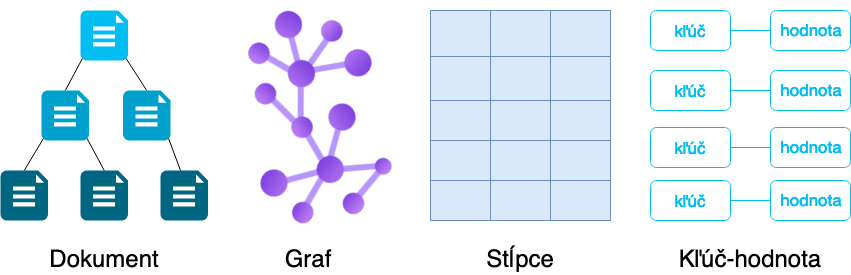
\includegraphics[scale=0.45]{obrazky/nosql_types.png}
        \caption{Ilustrácia typov NoSQL databáz \cite{nosql}.}
        \label{pic:nosql_types}
    \end{figure}

\section{Frontend}
Frontend, alebo častokrát nazývaný aj ako klient, je prezenčná vrstva aplikácie ktorá poskytuje používateľské rozhranie. Je to časť ktorú užívateľ vidí, s ktorou pracuje a ovláda. Medzi najpopulárnejšie technológie pre vývoj frontendu patrí HTML, CSS a JavaScript, pomocou ktorých je táto aplikácia implementovaná. 

\subsection{JavaScript}
JavaScript je objektovo orientovaný skriptovací jazyk. Najviac sa používa pri vývoji dynamických webových aplikácií, ale využíva sa aj pri tvorbe multiplatformových stolových aplikácií a hybridných mobilných aplikácií. Poskytuje interaktivitu nad obsahom. 

Medzi jeho výhody patrí dynamické načítanie stránky, zmena obsahu bez fyzického znova načítania stránky a rozšíriteľnosť. JavaScript sa hlavne zameriaval na klientskú časť aplikácie, kým nenastúpil na scénu framework \texttt{Node.js}\ref{node} a podobné serverové technológie, účelom ktorých je tvorba serverovej časti aplikácie.

Existuje niekoľko frameworkov pre uľahčenie vývoja, pomocou ktorých sa vyhneme takzvaným biolerplate\footnote{Biolerplate - kód ktorý sa musí opakovane vyskytovať na viacerých miestach bez významnej zmeny} kódom. Medzi najpopulárnejšie frameworky patrí Vue.js, React, Angular a Node.js.

\subsection{React}
React je frontendová JavaScriptová open-source\footnote{Open-source software má dostupný zdrojový kód pre verejnosť} knihovňa pre tvorbu užívateľských rozhraní. Na rozdiel od podobných frameworkov ako Angular, React sa sústreďuje iba na jednu špecifickú oblasť \textit{MVC}\footnote{Model-View-Controller - softwarová architektúra, ktorá rozdeľuje aplikáciu na dátový model, užívateľské rozhranie a logiku} architektúry, a to je vrstva pohľadu (anglicky \texttt{view}). Knihovňa bola predstavená v roku 2013 spoločnosťou Facebook, ktorá ju už niekoľko rokov pred tým používala a vyvíjala. 

\subsection{Angular}
Angular je JavaScriptový open-source framework, vytvorený spoločnostou Google. Súčasná verzia sa označuje aj ako Angular 2+, ktorá má zatiaľ jedenásť podverzií. Angular funguje na báze TypeScriptu o ktorom si povieme viac v kapitole \ref{typescript}.

\section{Backend}
Backend, mnohokrát nazývaný aj ako server, je základom aplikácie. Tvorí časť, ktorá je skrytá pred používateľom. Jeho úlohou je prijímanie a posielanie údajov od klienta cez API. Tieto údaje spracuje, ukladá, alebo modifikuje v databáze. 

\subsection{Firebase}
Firebase je platforma typu \textit{backend-ako-služba} (anglicky \texttt{Backend-as-a-Service}) , ktorá bola vytvorená v roku 2011. V roku 2014 bola odkúpená spoločnosťou Google, ktorá ju doteraz vyvíja. Pomáha v tvorbe, vylepšovaní, a škálovaní aplikácií.

BaaS je typ cloudových služieb pre tvorbu aplikácií bez investovania do vlastnej backend infraštruktúry. Uľahčuje vývojárom prácu zapúzdrením služieb na backendu, aby sa mohli sústrediť hlavne na tvorbu frontendu. Medzi ne patrí autentifikácia užívateľov, manažment databáze, monitorovanie a analýza, vzdialené aktualizácie, cloudové úložisko alebo hosting. Všetky tieto služby Firebase poskytuje. 

\subsection{Laravel}
Laravel je najpopulárnejší webový PHP framework vytvorený Taylorom Otwellom. Je založený na frameworku Symfony a má otvorený zrojový kód. Jeho použitie je bezplatné.

\subsection{Django}
Django je open-source webový framework pre vytváranie webových aplikácií. Je napísaný v programovacom jazyku Python. Používa princíp MTV (Model-Template-View), interpretovanú verziu MVC architektúry, ktorá obsahuje dátový model a pohľad ktorý je posielaný do šablóny. Namiesto písaní SQL dotazov preferuje prístup ORM, transformáciu Python objektov na dotazy.

\subsection{Spring boot}
TODO 

\subsection{ASP.NET Core}
ASP.NET Core je bezplatný webový framework vyvinutý a udržiavaný spoločnosťou Microsoft. Je nástupca technológie ASP.NET
TODO

\section{Slideshow framework}
Slideshow framework je nástroj pre vytváranie prezentácií vo webovom prehliadači pomocou webových technológií ako HTML, CSS a JavaScript.

\subsection{Eagle.js}
Eagle.js je slideshow framework založený na Vue.js. Podporuje animácie a motívy. Poskytuje užívateľom zopár komunitou vytvorených šablónov pre rýchlejšiu tvorbu prezentácií. 

Nevýhodou Eagle.js je, že jeho vývoj je zanedbaný. Posledná aktualizácia bola vydaná 23.10.2019. Framework používa takzvané mixiny, ktoré sú už v najnovšej verzii Vue.js neschválené (anglicky deprecated) a nahradené \texttt{Composition API}. O mixinoch a Composition API sa čitateľ dozvie viac v sekcii \ref{compositionapi}.

\subsection{Impress.js}
Impress.js je framework pre tvorbu prezentácií, bol inšpirovaný nápadom za prezi.com. Silnou stránkou tohto frameworku sú animácie poskytované CSS3.
TODO